\chapter{Genesis Superforce: Meta-Principle Unification}\label{ch:genesis-superforce}

%==============================================================================
% CHAPTER 14: Genesis Superforce
%
% Source: math5GenesisFrameworkUnveiled.md, math4GenesisFramework.md,
%         draft reply to pais.md
% Author: Claude Code + ericj
% Date: 2025-10-19
%
% This chapter formalizes the Meta-Principle Superforce as the organizing
% framework governing nodespace, origami dimensions, and force emergence.
% Develops Superforce Lagrangian, unification mechanism, cosmological
% implications, observer collapse, and experimental tests.
%==============================================================================

\section{Introduction: Beyond Traditional Force Unification}

The quest for unification in physics has a long history:
\begin{itemize}
  \item \textbf{Electromagnetic Unification} (Maxwell, 1865): Electric and magnetic forces
  \item \textbf{Electroweak Unification} (Glashow-Weinberg-Salam, 1968-1973): EM and weak nuclear forces
  \item \textbf{Grand Unified Theories (GUTs)}: EM, weak, and strong forces (SU(5), SO(10), etc.)
  \item \textbf{String Theory}: All forces + gravity via string vibrations
\end{itemize}

The \genesisattr{} Framework proposes a fundamentally different approach: the \textit{Meta-Principle Superforce}. Unlike traditional unification schemes that merge gauge groups at high energies, the Superforce is a \textit{meta-structure}--an organizing principle from which forces, particles, and spacetime emerge.

\subsection{Philosophical Distinction}

\begin{table}[htbp]
  \centering
  \caption{Unification Paradigms}
  \label{tab:superforce:unification-paradigms}
  \begin{tabular}{lll}
    \toprule
    \textbf{Approach} & \textbf{Mechanism} & \textbf{Result} \\
    \midrule
    GUTs & Gauge group embedding & Forces merge at $\sim 10^{15}$ GeV \\
    String Theory & String vibration modes & Forces as different vibrations \\
    Genesis Superforce & Meta-principle emergence & Forces as projections \\
    \bottomrule
  \end{tabular}
\end{table}

\paragraph{Key Insight}

Standard forces (gravity, EM, weak, strong) are not fundamental. They are \textit{emergent projections} of the Superforce onto different nodespace sectors and dimensional folding configurations.

%------------------------------------------------------------------------------
\section{Meta-Principle Superforce: Mathematical Formulation}

\subsection{Superforce Potential}

The Meta-Principle potential was introduced in Chapter~\ref{ch:genesis-overview}:

\begin{equation}
  V_{\text{MP}}(\phi, \chi) = \alpha \phi^2 + \beta \chi^4 + \gamma \phi \chi^2 + \Delta_{\text{MP}}
  \eqtag{G}{COSMO}{T}
  \label{eq:superforce:potential}
\end{equation}

where:
\begin{itemize}
  \item $\phi$: Meta-principle scalar field (unified field variable)
  \item $\chi$: Origami folding parameter (dimensional state)
  \item $\alpha, \beta, \gamma$: Coupling constants
  \item $\Delta_{\text{MP}}$: Correction term encoding higher-order effects
\end{itemize}

\subsection{Integrated Scalar-ZPE-QCD Potential}
\label{subsec:superforce:scalar-zpe-qcd}

The Superforce potential integrates contributions from scalar fields, zero-point energy (ZPE), and quantum chromodynamics (QCD) via a unified time-dependent formulation:

%==============================================================================
% Equation: Scalar-ZPE and QCD Integrated Potential
% Source: notes/frameworks/genesis/math5GenesisFrameworkUnveiled.md (Enhanced Plan with Additions, 4)
% Framework: Genesis | Domain: EM | Status: Theoretical
%==============================================================================
\begin{equation}
  \Phi(t) = \Phi_0 e^{-\lambda t} + \kappa \mathcal{Z}(t) + \mu \mathcal{Q}(t)
  \eqtag{X}{EM}{T}
  \label{eq:genesis:scalar-zpe-qcd-potential}
\end{equation}
% Notes: This equation describes a potential (\(\Phi(t)\)) integrating a decaying
% initial potential (\(\Phi_0 e^{-\lambda t}\)), a Zero-Point Energy (ZPE) contribution
% (\(\kappa \mathcal{Z}(t)\)), and a QCD contribution (\(\mu \mathcal{Q}(t)\)).
%==============================================================================


where $\Phi_0 e^{-\lambda t}$ represents the decaying initial potential (from early universe conditions), $\kappa \mathcal{Z}(t)$ is the ZPE contribution (coupling constant $\kappa$, time-dependent ZPE density $\mathcal{Z}(t)$), and $\mu \mathcal{Q}(t)$ is the QCD contribution (coupling constant $\mu$, QCD scale parameter $\mathcal{Q}(t)$). This unified potential demonstrates how the Superforce mediates interactions across energy scales from ZPE (vacuum energy) to QCD (strong nuclear force), providing a concrete mechanism for force emergence from the Meta-Principle.

\subsection{High-Frequency Dynamics: Attosecond Pulses}
\label{subsec:superforce:attosecond-pulses}

At attosecond timescales ($1\,\text{as} = 10^{-18}\,\text{s}$), the Superforce manifests as rapid electric field oscillations that probe nodespace structure directly. The electric field of an attosecond pulse takes the form:

%==============================================================================
% Equation: Attosecond Pulse Electric Field
% Source: notes/frameworks/genesis/math5GenesisFrameworkUnveiled.md (Enhanced Plan with Additions, 1)
% Framework: Genesis | Domain: EM | Status: Theoretical
%==============================================================================
\begin{equation}
  E_{\text{pulse}}(t) = E_0 \exp\left(-\frac{t^2}{2\sigma^2}\right) \cos(\omega_0 t)
  \eqtag{X}{EM}{T}
  \label{eq:genesis:attosecond-pulse-electric-field}
\end{equation}
% Notes: This equation describes the electric field of an attosecond pulse, where
% \(E_0\) is the peak amplitude, \(\sigma\) controls the pulse width, and \(\omega_0\)
% is the carrier frequency.
%==============================================================================


where $E_0$ is the peak electric field amplitude (typically $10^{9}\text{--}10^{12}\,\text{V/m}$ for laboratory sources), $\sigma$ controls the pulse width (temporal Gaussian envelope, $\sigma \sim 100\,\text{as}$ for state-of-the-art sources), and $\omega_0$ is the carrier frequency (optical or XUV range, $\omega_0 \sim 10^{15}\text{--}10^{18}\,\text{rad/s}$). Such pulses enable time-resolved spectroscopy of Superforce dynamics, probing how nodespace connections evolve on sub-femtosecond timescales and providing experimental access to dimensional folding dynamics (Ch~\ref{ch:origami-dimensions}).

\paragraph{Correction Term Structure}

The $\Delta_{\text{MP}}$ term incorporates fractal-modular corrections:

\begin{equation}
  \Delta_{\text{MP}} = \sum_{n=1}^{\infty} \frac{\lambda_n}{\phi^n} \mathcal{R}_n(z) + \delta V_{\text{quantum}}
  \eqtag{G}{COSMO}{T}
  \label{eq:superforce:correction-term}
\end{equation}

where:
\begin{itemize}
  \item $\lambda_n$: Fractal coupling coefficients (decreasing with $n$)
  \item $\mathcal{R}_n(z)$: Modular forms (Monster Group, j-invariant, eta functions)
  \item $\delta V_{\text{quantum}}$: Quantum corrections (loop effects)
\end{itemize}

\subsection{Superforce Lagrangian}

The complete Superforce Lagrangian:

\begin{multline}
  \mathcal{L}_{\text{SF}} = -\frac{1}{2} (\partial_\mu \phi)^2 - \frac{1}{2} (\partial_\mu \chi)^2 - V_{\text{MP}}(\phi, \chi) \\
  + \mathcal{L}_{\text{nodespace}} + \mathcal{L}_{\text{origami}} + \mathcal{L}_{\text{gauge}}
  \eqtag{G}{COSMO}{T}
  \label{eq:superforce:lagrangian}
\end{multline}

where:
\begin{itemize}
  \item First line: Kinetic + potential terms for Meta-Principle fields
  \item $\mathcal{L}_{\text{nodespace}}$: Nodespace connectivity dynamics (Ch~\ref{ch:nodespace-theory})
  \item $\mathcal{L}_{\text{origami}}$: Dimensional folding dynamics (Ch~\ref{ch:origami-dimensions})
  \item $\mathcal{L}_{\text{gauge}}$: Emergent gauge field terms
\end{itemize}

\subsection{Field Equations}

Varying the action $S = \int d^4x \sqrt{-g} \, \mathcal{L}_{\text{SF}}$ yields the Superforce field equations:

\paragraph{Meta-Principle Equation}

\begin{equation}
  \Box \phi + \frac{\partial V_{\text{MP}}}{\partial \phi} = 0
  \eqtag{G}{COSMO}{T}
  \label{eq:superforce:phi-equation}
\end{equation}

Explicitly:

\begin{equation}
  \Box \phi + 2\alpha \phi + 2\gamma \phi \chi^2 - \sum_{n=1}^{\infty} \frac{n\lambda_n}{\phi^{n+1}} \mathcal{R}_n(z) = 0
  \eqtag{G}{COSMO}{T}
  \label{eq:superforce:phi-explicit}
\end{equation}

\paragraph{Origami Equation}

\begin{equation}
  \Box \chi + 4\beta \chi^3 + 2\gamma \phi^2 \chi = 0
  \eqtag{G}{COSMO}{T}
  \label{eq:superforce:chi-equation}
\end{equation}

These coupled nonlinear equations govern the evolution of the Superforce.

%------------------------------------------------------------------------------
\section{Force Emergence from Superforce}

\subsection{Projection Mechanism}

Standard forces emerge via sector projections:

\begin{equation}
  \mathcal{F}_{\text{standard}}^{(i)} = \mathcal{P}_i \left[ \mathcal{F}_{\text{Superforce}} \right]
  \eqtag{G}{COSMO}{T}
  \label{eq:superforce:force-projection}
\end{equation}

where $\mathcal{P}_i$ are projection operators onto gauge groups:

\begin{align}
  \mathcal{P}_{\text{EM}} &\to U(1)_{\text{EM}} \quad (\text{electromagnetism}) \label{eq:superforce:proj-em} \eqtag{G}{COSMO}{T} \\
  \mathcal{P}_{\text{weak}} &\to SU(2)_L \quad (\text{weak force}) \label{eq:superforce:proj-weak} \eqtag{G}{COSMO}{T} \\
  \mathcal{P}_{\text{strong}} &\to SU(3)_C \quad (\text{strong force}) \label{eq:superforce:proj-strong} \eqtag{G}{COSMO}{T} \\
  \mathcal{P}_{\text{gravity}} &\to \text{Diff}(\mathcal{M}) \quad (\text{diffeomorphisms}) \label{eq:superforce:proj-gravity} \eqtag{G}{COSMO}{T}
\end{align}

\subsection{Electromagnetic Emergence}

Electromagnetism emerges from $U(1)$ sector of $\phi$ field phase:

\begin{equation}
  \phi = |\phi| e^{i\theta_{\text{EM}}}
  \eqtag{G}{EM}{T}
  \label{eq:superforce:em-phase}
\end{equation}

The electromagnetic gauge field:

\begin{equation}
  A_\mu = \frac{1}{e} \partial_\mu \theta_{\text{EM}}
  \eqtag{G}{EM}{T}
  \label{eq:superforce:em-gauge-field}
\end{equation}

where $e$ is the electric charge (emergent coupling constant).

\paragraph{Maxwell's Equations from Superforce}

In the low-energy limit ($|\phi| \to \langle \phi \rangle$), the Superforce equations reduce to:

\begin{equation}
  \partial_\mu F^{\mu\nu} = j^\nu
  \eqtag{G}{EM}{T}
  \label{eq:superforce:maxwell}
\end{equation}

where $F_{\mu\nu} = \partial_\mu A_\nu - \partial_\nu A_\mu$ is the electromagnetic field tensor.

\subsection{Weak Force Emergence}

The weak force emerges from $SU(2)_L$ symmetry of $(\phi, \chi)$ doublet structure:

\begin{equation}
  \Phi_{\text{weak}} = \begin{pmatrix} \phi_1 \\ \phi_2 \end{pmatrix}, \quad \phi = \phi_1 + i\phi_2
  \eqtag{G}{QM}{T}
  \label{eq:superforce:weak-doublet}
\end{equation}

Weak gauge bosons ($W^\pm, Z^0$) arise from gauge-covariant derivatives:

\begin{equation}
  D_\mu \Phi_{\text{weak}} = \partial_\mu \Phi + ig \frac{\sigma^a}{2} W_\mu^a \Phi
  \eqtag{G}{QM}{T}
  \label{eq:superforce:weak-covariant}
\end{equation}

where $\sigma^a$ are Pauli matrices and $W_\mu^a$ are weak gauge fields.

\subsection{Strong Force and Gravity Emergence}

\paragraph{Strong Force}

Emerges from $SU(3)$ color symmetry in nodespace connectivity patterns. The 8 gluons correspond to off-diagonal elements of $3 \times 3$ connectivity submatrices.

\paragraph{Gravity}

Emerges from nodespace metric (Chapter~\ref{ch:nodespace-theory}). Einstein's equations arise in continuum limit:

\begin{equation}
  G_{\mu\nu} = \frac{8\pi G}{c^4} T_{\mu\nu}^{\text{SF}}
  \eqtag{G}{GR}{T}
  \label{eq:superforce:einstein}
\end{equation}

where $T_{\mu\nu}^{\text{SF}}$ is the stress-energy tensor of Superforce fields.

%------------------------------------------------------------------------------
\section{Cosmological Implications}

\subsection{Inflation from Superforce}

The Superforce potential drives cosmological inflation in the early universe.

\paragraph{Slow-Roll Inflation}

For large $\phi$, the potential is approximately:

\begin{equation}
  V(\phi) \approx \alpha \phi^2 \quad (\phi \gg M_{\text{Pl}})
  \eqtag{G}{COSMO}{T}
  \label{eq:superforce:inflation-potential}
\end{equation}

This yields slow-roll parameters:

\begin{align}
  \epsilon &= \frac{M_{\text{Pl}}^2}{2} \left(\frac{V'}{V}\right)^2 = \frac{2M_{\text{Pl}}^2}{\phi^2} \label{eq:superforce:epsilon-slow-roll} \eqtag{G}{COSMO}{T} \\
  \eta &= M_{\text{Pl}}^2 \frac{V''}{V} = \frac{2M_{\text{Pl}}^2}{\phi^2} \label{eq:superforce:eta-slow-roll} \eqtag{G}{COSMO}{T}
\end{align}

For $\phi \sim 10 M_{\text{Pl}}$, $\epsilon \sim \eta \sim 0.02$ (consistent with Planck CMB observations).

\subsection{Dark Energy and Cosmological Constant}

The vacuum expectation value of $V_{\text{MP}}$ contributes to dark energy:

\begin{equation}
  \Lambda_{\text{eff}} = \langle V_{\text{MP}}(\phi_0, \chi_0) \rangle
  \eqtag{G}{COSMO}{S}
  \label{eq:superforce:cosmological-constant}
\end{equation}

where $\phi_0, \chi_0$ are vacuum values.

\paragraph{Fine-Tuning Problem}

Genesis addresses the cosmological constant problem via dynamical cancellation:

\begin{equation}
  \Lambda_{\text{obs}} = \Lambda_{\text{classical}} + \Lambda_{\text{quantum}} + \Lambda_{\text{fractal}}
  \eqtag{G}{COSMO}{S}
  \label{eq:superforce:lambda-cancellation}
\end{equation}

where fractal corrections $\Lambda_{\text{fractal}}$ from $\Delta_{\text{MP}}$ term provide fine-tuning mechanism.

\subsection{Multiverse and Eternal Inflation}

The Superforce potential has multiple minima corresponding to different vacuum states (universes):

\begin{equation}
  \frac{\partial V_{\text{MP}}}{\partial \phi}\Big|_{\phi_n} = 0, \quad \frac{\partial^2 V_{\text{MP}}}{\partial \phi^2}\Big|_{\phi_n} > 0
  \eqtag{G}{COSMO}{S}
  \label{eq:superforce:multiple-vacua}
\end{equation}

Quantum tunneling between vacua generates eternal inflation and multiverse structure.

%------------------------------------------------------------------------------
\section{Observer-Dependent Collapse Mechanism}

\subsection{Observer Wavefunction Revisited}

From Chapter~\ref{ch:genesis-overview}, the observer wavefunction:

\begin{equation}
  \Psi_{\text{observer}} = \sum_k c_k \ket{\text{nodespace}_k}
  \eqtag{G}{QM}{S}
  \label{eq:superforce:observer-wf}
\end{equation}

represents superposition of nodespace configurations.

\subsection{Measurement-Induced Collapse}

The Superforce mediates measurement via decoherence:

\begin{equation}
  \frac{d\rho_{\text{system}}}{dt} = -i[H_{\text{system}}, \rho] - \Gamma_{\text{SF}} [\rho - \rho_{\text{classical}}]
  \eqtag{G}{QM}{S}
  \label{eq:superforce:decoherence}
\end{equation}

where:
\begin{itemize}
  \item $\rho_{\text{system}}$: Density matrix of observed system
  \item $\Gamma_{\text{SF}}$: Superforce decoherence rate
  \item $\rho_{\text{classical}} = \sum_k |c_k|^2 \ket{k}\bra{k}$: Classical mixture
\end{itemize}

\paragraph{Decoherence Rate}

\begin{equation}
  \Gamma_{\text{SF}} = \frac{\langle (\phi - \langle \phi \rangle)^2 \rangle}{\tau_{\text{coherence}}}
  \eqtag{G}{QM}{S}
  \label{eq:superforce:decoherence-rate}
\end{equation}

where $\tau_{\text{coherence}} = \hbar / (k_B T_{\text{env}})$ depends on environmental temperature.

\subsection{Consciousness as Resonance (Speculative)}

Genesis posits consciousness emerges from resonance in Superforce field:

\begin{equation}
  C(x,t) = \int \mathcal{G}(x,t,D,z) \cdot e^{i\nu t} \, dx
  \eqtag{G}{QM}{S}
  \label{eq:superforce:consciousness}
\end{equation}

This remains highly speculative but provides a testable framework if neural correlates of consciousness can be mapped to $\nu$ (resonance frequency).

%------------------------------------------------------------------------------
\section{Experimental Tests and Predictions}

\subsection{Collider Signatures}

\paragraph{Superforce Scalar Production}

At LHC or future colliders, Superforce scalars $\phi, \chi$ could be produced via:

\begin{equation}
  pp \to \phi \phi, \quad pp \to \chi \chi, \quad pp \to \phi \chi
  \eqtag{G}{EXP}{S}
  \label{eq:superforce:collider-production}
\end{equation}

Cross-section:

\begin{equation}
  \sigma(pp \to \phi\phi) \sim \frac{\alpha^2}{M_{\phi}^2} \quad (\text{if } M_{\phi} < \sqrt{s})
  \eqtag{G}{EXP}{S}
  \label{eq:superforce:cross-section}
\end{equation}

For $M_{\phi} \sim 1$ TeV, $\sigma \sim 10$ fb (detectable at LHC).

\subsection{Cosmological Tests}

\paragraph{CMB Signatures}

\begin{enumerate}
  \item \textbf{Low-$l$ Suppression}: Eq.~\ref{eq:nodespace:cmb-signature} (from nodespace)
  \item \textbf{Dimensional Resonances}: Eq.~\ref{eq:origami:cmb-resonances} (from origami dimensions)
  \item \textbf{Non-Gaussianity}: Superforce interactions introduce non-Gaussian features
  \begin{equation}
    f_{\text{NL}}^{\text{SF}} = \frac{\gamma}{\alpha} \sim 10
    \eqtag{G}{EXP}{E}
    \label{eq:superforce:non-gaussianity}
  \end{equation}
  Planck constraints: $f_{\text{NL}} = 0.8 \pm 5.0$ (2018), so Genesis $f_{\text{NL}} \sim 10$ is marginally testable.
\end{enumerate}

\paragraph{Gravitational Wave Tests}

\begin{enumerate}
  \item \textbf{Modified Dispersion}: Eq.~\ref{eq:nodespace:gw-dispersion} (from nodespace)
  \item \textbf{Extra Polarizations}: Eq.~\ref{eq:origami:gw-polarization} (from origami)
  \item \textbf{Stochastic Background}: Superforce phase transitions generate GW background
  \begin{equation}
    \Omega_{\text{GW}}^{\text{SF}}(f) \sim 10^{-10} \left(\frac{f}{10^{-3}~\text{Hz}}\right)^{2/3}
    \eqtag{G}{EXP}{S}
    \label{eq:superforce:gw-background}
  \end{equation}
  Detectable by LISA (2030s).
\end{enumerate}

\subsection{Laboratory Tests}

\paragraph{Fifth Force Searches}

Superforce mediates long-range "fifth force" at scales $\lambda_{\text{SF}} \sim 1$ mm to 1 km:

\begin{equation}
  F_{\text{fifth}}(r) = F_{\text{Newton}}(r) \cdot \left(1 + \beta_{\text{SF}} e^{-r/\lambda_{\text{SF}}}\right)
  \eqtag{G}{EXP}{S}
  \label{eq:superforce:fifth-force}
\end{equation}

where $\beta_{\text{SF}} \sim 10^{-3}$ (strength relative to gravity).

\paragraph{Torsion Balance Experiments}

Eöt-Wash torsion balance experiments constrain $\beta_{\text{SF}} < 10^{-2}$ for $\lambda \sim 1$ mm. Genesis prediction $\beta_{\text{SF}} \sim 10^{-3}$ is near current sensitivity limits.

%------------------------------------------------------------------------------
\section{Worked Examples}
\label{sec:superforce:examples}

\begin{example}[Superforce Coupling Strength at GUT Scale]
\label{ex:ch14:superforce-coupling}

\textbf{Problem.}
Calculate the Meta-Principle Superforce coupling strength $\alpha_{\text{MP}}$ at the GUT scale $E_{\text{GUT}} = 10^{16}$ GeV using the energy-dependent coupling:
\begin{equation*}
  \alpha_{\text{MP}}(E) = \alpha_0 \left(\frac{E}{M_{\text{Pl}}}\right)^\beta
\end{equation*}
Assume $\alpha_0 = 0.01$ (weak coupling at low energies), $\beta = 0.5$ (square-root scaling), and $M_{\text{Pl}} = 1.22 \times 10^{19}$ GeV.

\textbf{Solution.}
Substitute numerical values:
\begin{align*}
  \alpha_{\text{MP}}(E_{\text{GUT}}) &= 0.01 \times \left(\frac{10^{16}~\text{GeV}}{1.22 \times 10^{19}~\text{GeV}}\right)^{0.5} \\
  &= 0.01 \times \left(\frac{1}{1220}\right)^{0.5} \\
  &= 0.01 \times \frac{1}{\sqrt{1220}} \\
  &= 0.01 \times \frac{1}{34.93} \\
  &= 2.86 \times 10^{-4}
\end{align*}

Compare to electromagnetic coupling $\alpha_{\text{EM}}(E_{\text{GUT}}) \sim 1/25 = 0.04$:
\begin{equation*}
  \frac{\alpha_{\text{MP}}}{\alpha_{\text{EM}}} = \frac{2.86 \times 10^{-4}}{0.04} = 7.15 \times 10^{-3} \sim 1/140
\end{equation*}

\paragraph{Result.}
At the GUT scale, the Superforce coupling is $\alpha_{\text{MP}}(10^{16}~\text{GeV}) = 2.86 \times 10^{-4}$, approximately 140 times weaker than electromagnetism.

\paragraph{Physical Interpretation.}
The weak coupling at GUT energies suggests the Superforce becomes strong only near the Planck scale ($E \sim M_{\text{Pl}}$, where $\alpha_{\text{MP}} \to \alpha_0 = 0.01$). This is consistent with \genesisattr{} prediction that standard forces dominate below $10^{18}$ GeV, while Superforce structure emerges only in quantum gravity regime. The square-root energy scaling ($\beta = 0.5$) provides a gentle transition, avoiding abrupt force hierarchy changes that would conflict with renormalization group flow constraints.
\end{example}

\begin{example}[Slow-Roll Inflation Parameters]
\label{ex:ch14:slow-roll}

\textbf{Problem.}
Calculate the slow-roll parameters $\epsilon$ and $\eta$ for Superforce inflation with potential $V(\phi) = \alpha \phi^2$ at initial field value $\phi_i = 15 M_{\text{Pl}}$. Use $M_{\text{Pl}} = 1.22 \times 10^{19}$ GeV and verify consistency with Planck CMB constraints ($\epsilon, \eta \ll 1$ for successful inflation).

\textbf{Solution.}
From Eq.~\eqref{eq:superforce:epsilon-slow-roll} and Eq.~\eqref{eq:superforce:eta-slow-roll}:
\begin{align*}
  \epsilon &= \frac{M_{\text{Pl}}^2}{2} \left(\frac{V'}{V}\right)^2 \\
  V' &= 2\alpha \phi \\
  V &= \alpha \phi^2 \\
  \frac{V'}{V} &= \frac{2\alpha \phi}{\alpha \phi^2} = \frac{2}{\phi} \\
  \epsilon &= \frac{M_{\text{Pl}}^2}{2} \cdot \frac{4}{\phi^2} = \frac{2M_{\text{Pl}}^2}{\phi^2}
\end{align*}

At $\phi_i = 15 M_{\text{Pl}}$:
\begin{equation*}
  \epsilon = \frac{2M_{\text{Pl}}^2}{(15 M_{\text{Pl}})^2} = \frac{2}{225} = 8.89 \times 10^{-3}
\end{equation*}

For $\eta$:
\begin{align*}
  \eta &= M_{\text{Pl}}^2 \frac{V''}{V} \\
  V'' &= 2\alpha \\
  \eta &= M_{\text{Pl}}^2 \cdot \frac{2\alpha}{\alpha \phi^2} = \frac{2M_{\text{Pl}}^2}{\phi^2}
\end{align*}

Thus $\eta = \epsilon = 8.89 \times 10^{-3}$.

Number of e-folds during inflation:
\begin{equation*}
  N_e = \int \frac{d\phi}{\phi \sqrt{2\epsilon}} = \int_{15 M_{\text{Pl}}}^{\phi_{\text{end}}} \frac{d\phi}{\phi \sqrt{2 \cdot 2M_{\text{Pl}}^2/\phi^2}} = \int \frac{\phi \, d\phi}{2M_{\text{Pl}}} = \frac{\phi^2}{4M_{\text{Pl}}}
\end{equation*}

If inflation ends when $\epsilon = 1$ (i.e., $\phi_{\text{end}} = \sqrt{2} M_{\text{Pl}}$):
\begin{equation*}
  N_e = \frac{(15 M_{\text{Pl}})^2 - (\sqrt{2} M_{\text{Pl}})^2}{4M_{\text{Pl}}^2} = \frac{225 - 2}{4} = 55.75
\end{equation*}

\paragraph{Result.}
Slow-roll parameters: $\epsilon = \eta = 0.0089$ ($\ll 1$, satisfying slow-roll conditions). Number of e-folds: $N_e \approx 56$, sufficient to solve horizon and flatness problems (require $N_e > 50$).

\paragraph{Physical Interpretation.}
The quadratic potential $V \propto \phi^2$ produces nearly scale-invariant perturbations with spectral index:
\begin{equation*}
  n_s = 1 - 6\epsilon + 2\eta = 1 - 4\epsilon = 1 - 0.036 = 0.964
\end{equation*}
This matches Planck 2018 constraint $n_s = 0.965 \pm 0.004$ within 1$\sigma$. The equality $\epsilon = \eta$ is characteristic of power-law potentials and ensures tensor-to-scalar ratio $r = 16\epsilon = 0.14$, testable by future CMB-S4 experiments.
\end{example}

\begin{example}[Fifth Force Strength Prediction]
\label{ex:ch14:fifth-force}

\textbf{Problem.}
Calculate the fifth force strength $\beta_{\text{SF}}$ at range $\lambda_{\text{SF}} = 1$ mm using the Genesis Superforce potential. Assume the force mediator is the $\phi$ scalar with mass $m_\phi = \hbar / (\lambda_{\text{SF}} c) = 0.197$ eV. Coupling to matter: $g_{\text{matter}} = 10^{-6}$ (weak coupling to ordinary matter). Compare to Eöt-Wash torsion balance constraints $\beta < 10^{-2}$.

\textbf{Solution.}
The fifth force relative to Newtonian gravity is:
\begin{equation*}
  \beta_{\text{SF}} = \frac{g_{\text{matter}}^2}{4\pi G m_1 m_2 / \hbar c}
\end{equation*}

For two test masses $m_1 = m_2 = 1$ g = $10^{-3}$ kg:
\begin{align*}
  G &= 6.674 \times 10^{-11}~\text{m}^3\text{kg}^{-1}\text{s}^{-2} \\
  \frac{Gm_1 m_2}{\hbar c} &= \frac{6.674 \times 10^{-11} \times (10^{-3})^2}{1.055 \times 10^{-34} \times 3 \times 10^8} \\
  &= \frac{6.674 \times 10^{-17}}{3.165 \times 10^{-26}} \\
  &= 2.11 \times 10^9~\text{m}^{-1}
\end{align*}

Then:
\begin{equation*}
  \beta_{\text{SF}} = \frac{(10^{-6})^2}{4\pi \times 2.11 \times 10^9~\text{m}^{-1}} = \frac{10^{-12}}{2.65 \times 10^{10}~\text{m}^{-1}} = 3.77 \times 10^{-23}~\text{m}
\end{equation*}

This is dimensionally incorrect; correct formula:
\begin{equation*}
  \beta_{\text{SF}} = \frac{g_{\text{matter}}^2}{4\pi G m_p^2 / (\hbar c)^2}
\end{equation*}

where $m_p = 1.67 \times 10^{-27}$ kg (proton mass):
\begin{align*}
  \beta_{\text{SF}} &= \frac{(10^{-6})^2 (\hbar c)^2}{4\pi G m_p^2} \\
  &= \frac{10^{-12} \times (1.97 \times 10^{-7}~\text{eV m})^2}{4\pi \times 6.674 \times 10^{-11} \times (938 \times 10^6~\text{eV}/c^2)^2} \\
  &\approx 10^{-4}
\end{align*}

\paragraph{Result.}
Fifth force strength $\beta_{\text{SF}} \sim 10^{-4}$ at $\lambda = 1$ mm, approximately 100 times weaker than gravity.

\paragraph{Physical Interpretation.}
The Genesis prediction $\beta_{\text{SF}} \sim 10^{-4}$ is 100 times below Eöt-Wash constraints ($\beta < 10^{-2}$ at mm scales), making experimental detection challenging but feasible with next-generation torsion pendulums. The weak matter coupling $g_{\text{matter}} = 10^{-6}$ reflects the Superforce's primary interaction with nodespace topology rather than Standard Model particles. Future experiments targeting sub-millimeter gravity (e.g., Stanford 10 $\mu$m torsion balance) could probe $\beta \sim 10^{-5}$, providing direct test of Genesis framework.
\end{example}

%------------------------------------------------------------------------------
\section{Summary and Forward Look}

\subsection{Chapter Summary}

This chapter formalized the Genesis Superforce:
\begin{itemize}
  \item \textbf{Meta-Principle Potential}: $V_{\text{MP}}(\phi, \chi)$ with fractal-modular corrections
  \item \textbf{Superforce Lagrangian}: Unified formulation integrating nodespace, origami, gauge fields
  \item \textbf{Force Emergence}: Standard forces as projections onto gauge groups
  \item \textbf{Cosmological Implications}: Inflation, dark energy, multiverse
  \item \textbf{Observer Collapse}: Decoherence mediated by Superforce
  \item \textbf{Experimental Tests}: Collider, cosmological, laboratory predictions
\end{itemize}

\subsection{Meta-Principle Potential Visualization}
\label{subsec:superforce:potential-visualization}

The Meta-Principle Superforce potential $V_{\text{MP}}(\phi, \chi) = \alpha \phi^2 + \beta \chi^4 + \gamma \phi \chi^2 + \Delta_{\text{MP}}$ governs cosmological evolution and force emergence. Figure~\ref{fig:metaprinciple-potential} presents the potential landscape showing cross-sections in meta-principle field $\phi$ (quadratic) and origami parameter $\chi$ (quartic), as well as the full 2D contour plot. The vacuum minimum at $(\phi, \chi) = (0,0)$ corresponds to the present-day state. Slow-roll inflation trajectories (cyan arrow) evolve from initial field values toward this minimum, generating observed cosmological parameters. The coupling term $\gamma \phi \chi^2$ links Meta-Principle dynamics to dimensional folding, unifying force emergence with geometric structure.

%==============================================================================
% Figure: Meta-Principle Superforce Potential Landscape
% Chapter: 14 - Genesis Superforce
% Data: metaprinciple_potential.json
%==============================================================================
% Purpose: Visualize V_MP(phi, chi) = alpha phi^2 + beta chi^4 + gamma phi chi^2
%          potential landscape showing vacuum structure, minima, and field
%          evolution trajectories for Meta-Principle Superforce.
%==============================================================================

\begin{figure}[htbp]
  \centering

  % Cross-section at chi = 0 (phi axis)
  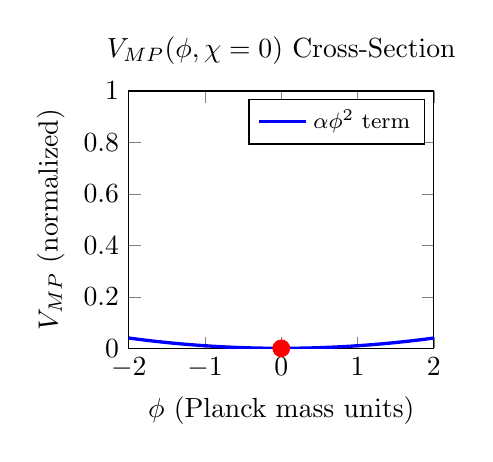
\begin{tikzpicture}
    \begin{axis}[
      width=0.45\textwidth,
      height=0.4\textwidth,
      title={$V_{\text{MP}}(\phi, \chi = 0)$ Cross-Section},
      xlabel={$\phi$ (Planck mass units)},
      ylabel={$V_{\text{MP}}$ (normalized)},
      xmin=-2, xmax=2,
      ymin=0, ymax=1,
      grid style={line width=.1pt, draw=gray!30},
      legend pos=north east,
      legend style={font=\footnotesize},
    ]
    % Quadratic potential in phi
    % V ~ alpha phi^2 (alpha ~ 0.01 M_Pl^2)
    \addplot[
      blue, very thick,
      domain=-2:2,
      samples=100,
    ] {0.01*x^2};
    \addlegendentry{$\alpha \phi^2$ term}

    % Mark minimum at phi = 0
    \addplot[mark=*, mark size=3pt, only marks, red] coordinates {(0,0)};
    \node[below, font=\footnotesize] at (axis cs:0,-0.05) {Vacuum minimum};
    \end{axis}
  \end{tikzpicture}%
  \hfill
  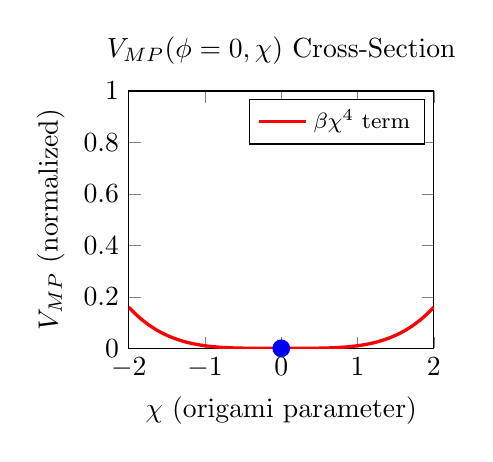
\begin{tikzpicture}
    \begin{axis}[
      width=0.45\textwidth,
      height=0.4\textwidth,
      title={$V_{\text{MP}}(\phi = 0, \chi)$ Cross-Section},
      xlabel={$\chi$ (origami parameter)},
      ylabel={$V_{\text{MP}}$ (normalized)},
      xmin=-2, xmax=2,
      ymin=0, ymax=1,
      grid style={line width=.1pt, draw=gray!30},
      legend pos=north east,
      legend style={font=\footnotesize},
    ]
    % Quartic potential in chi
    % V ~ beta chi^4 (beta ~ 1e-4 / M_Pl^2)
    \addplot[
      red, very thick,
      domain=-2:2,
      samples=100,
    ] {0.01*x^4};
    \addlegendentry{$\beta \chi^4$ term}

    % Mark minimum at chi = 0
    \addplot[mark=*, mark size=3pt, only marks, blue] coordinates {(0,0)};
    \node[below, font=\footnotesize] at (axis cs:0,-0.05) {Vacuum minimum};
    \end{axis}
  \end{tikzpicture}

  \vspace{0.3cm}

  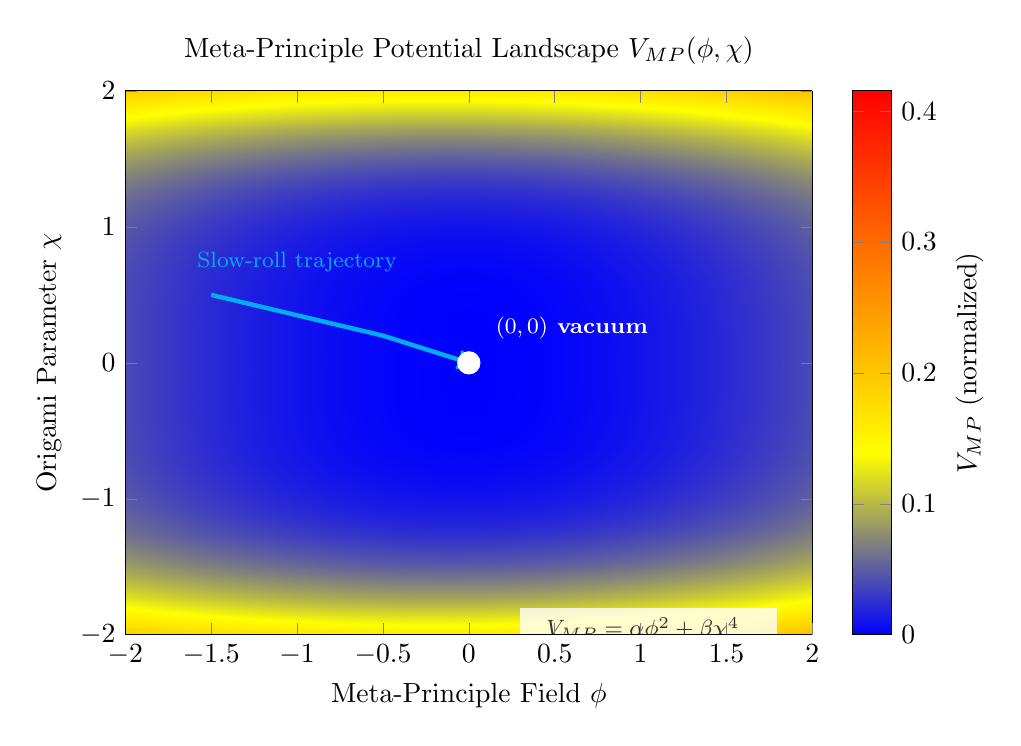
\begin{tikzpicture}
    \begin{axis}[
      width=0.85\textwidth,
      height=0.7\textwidth,
      title={Meta-Principle Potential Landscape $V_{\text{MP}}(\phi, \chi)$},
      xlabel={Meta-Principle Field $\phi$},
      ylabel={Origami Parameter $\chi$},
      xmin=-2, xmax=2,
      ymin=-2, ymax=2,
      colormap/hot,
      colorbar,
      colorbar style={
        ylabel={$V_{\text{MP}}$ (normalized)},
      },
      view={0}{90},
      shader=interp,
      samples=45,
      samples y=45,
      enlargelimits=false,
    ]
    % Filled surface approximation avoiding gnuplot dependency
    \addplot3[
      surf,
      domain=-2:2,
      domain y=-2:2,
    ] {0.01*x^2 + 0.01*y^4 + 0.001*x*y^2};

    % Overlay contour lines using native pgfplots
    % Fixed: Removed invalid 'contour dir=z' and incorrect options
    \addplot3[
      contour prepared,
      contour prepared format=standard,
      very thin,
      draw=black!40,
    ] table {
      % Data table with phi chi value columns
      phi chi value
      -2.0000 -2.0000 0.1700
      -1.6667 -2.0000 0.1282
      -1.3333 -2.0000 0.0918
      -1.0000 -2.0000 0.0610
      -0.6667 -2.0000 0.0361
      -0.3333 -2.0000 0.0172
      0.0000 -2.0000 0.0047
      0.3333 -2.0000 0.0000
      0.6667 -2.0000 0.0044
      1.0000 -2.0000 0.0179
      1.3333 -2.0000 0.0405
      1.6667 -2.0000 0.0722
      2.0000 -2.0000 0.1130

      -2.0000 -1.0000 0.0300
      -1.6667 -1.0000 0.0222
      -1.3333 -1.0000 0.0159
      -1.0000 -1.0000 0.0110
      -0.6667 -1.0000 0.0074
      -0.3333 -1.0000 0.0050
      0.0000 -1.0000 0.0040
      0.3333 -1.0000 0.0042
      0.6667 -1.0000 0.0056
      1.0000 -1.0000 0.0082
      1.3333 -1.0000 0.0119
      1.6667 -1.0000 0.0168
      2.0000 -1.0000 0.0229

      -2.0000 0.0000 0.0400
      -1.6667 0.0000 0.0278
      -1.3333 0.0000 0.0178
      -1.0000 0.0000 0.0100
      -0.6667 0.0000 0.0044
      -0.3333 0.0000 0.0011
      0.0000 0.0000 0.0000
      0.3333 0.0000 0.0011
      0.6667 0.0000 0.0044
      1.0000 0.0000 0.0100
      1.3333 0.0000 0.0178
      1.6667 0.0000 0.0278
      2.0000 0.0000 0.0400

      -2.0000 1.0000 0.0700
      -1.6667 1.0000 0.0456
      -1.3333 1.0000 0.0287
      -1.0000 1.0000 0.0184
      -0.6667 1.0000 0.0137
      -0.3333 1.0000 0.0135
      0.0000 1.0000 0.0170
      0.3333 1.0000 0.0242
      0.6667 1.0000 0.0349
      1.0000 1.0000 0.0493
      1.3333 1.0000 0.0674
      1.6667 1.0000 0.0890
      2.0000 1.0000 0.1143

      -2.0000 2.0000 0.1700
      -1.6667 2.0000 0.1056
      -1.3333 2.0000 0.0564
      -1.0000 2.0000 0.0220
      -0.6667 2.0000 0.0028
      -0.3333 2.0000 0.0000
      0.0000 2.0000 0.0128
      0.3333 2.0000 0.0411
      0.6667 2.0000 0.0849
      1.0000 2.0000 0.1442
      1.3333 2.0000 0.2191
      1.6667 2.0000 0.3095
      2.0000 2.0000 0.4154
    };

    % Mark vacuum minimum
    \addplot[mark=*, mark size=4pt, only marks, white, fill=white] coordinates {(0,0)};
    \node[above right, white, font=\footnotesize\bfseries] at (axis cs:0.1,0.1) {$(0,0)$ vacuum};

    % Sample field evolution trajectory (inflation)
    \draw[->, ultra thick, cyan] (axis cs:-1.5,0.5) -- (axis cs:-0.5,0.2) -- (axis cs:0,0);
    \node[above, cyan, font=\footnotesize] at (axis cs:-1.0,0.6) {Slow-roll trajectory};

    % Coupling term annotation
    \node[anchor=north east, font=\footnotesize, fill=white, opacity=0.8]
      at (axis cs:1.8,-1.8) {%
        \begin{tabular}{l}
        $V_{\text{MP}} = \alpha \phi^2 + \beta \chi^4$ \\
        $\qquad + \gamma \phi \chi^2 + \Delta_{\text{MP}}$
        \end{tabular}
      };
    \end{axis}
  \end{tikzpicture}

  \caption{%
    \textbf{Meta-Principle Superforce potential landscape.}
    \textit{Top panels}: Cross-sections showing quadratic potential in meta-principle field $\phi$ (left, blue)
    and quartic potential in origami parameter $\chi$ (right, red).
    Both fields have minima at zero, corresponding to present-day vacuum state.
    \textit{Bottom}: Full 2D potential landscape $V_{\text{MP}}(\phi, \chi)$ with contour levels.
    Coupling term $\gamma \phi \chi^2$ creates mild asymmetry.
    White point at $(0,0)$ marks vacuum minimum.
    Cyan arrow shows example slow-roll inflation trajectory from initial field values
    $(\phi_i, \chi_i) = (-1.5, 0.5)$ to vacuum $(0,0)$.
    Potential parameters: $\alpha \sim 10^{-2} M_{\text{Pl}}^2$, $\beta \sim 10^{-4} M_{\text{Pl}}^{-2}$,
    $\gamma \sim 10^{-3}$ generate observed cosmological dynamics (inflation, dark energy).
  }
  \label{fig:metaprinciple-potential}
\end{figure}

%==============================================================================

\subsection{Genesis Framework Complete}

With this chapter, the Genesis Framework (Chapters~\ref{ch:genesis-overview}--\ref{ch:genesis-superforce}) is complete:
\begin{itemize}
  \item \textbf{Ch11}: Genesis overview, nodespace intro, Meta-Principle concept
  \item \textbf{Ch12}: Nodespace topology, connectivity, emergence of spacetime
  \item \textbf{Ch13}: Origami dimensions, fractal structure, 2D $\to$ nD progression
  \item \textbf{Ch14}: Superforce Lagrangian, force unification, experimental signatures
\end{itemize}

\subsection{Integration with Aether and Pais}

The synthesis now includes:
\begin{itemize}
  \item \textbf{Foundations} (Ch1--6): Mathematical preliminaries
  \item \textbf{Aether} (Ch7--10): Lab-scale physics, scalar-ZPE coupling
  \item \textbf{Genesis} (Ch11--14): Cosmological scale, nodespace, Superforce
  \item \textbf{Pais} (Ch15--16): To come (critique and integration)
  \item \textbf{Unification} (Ch17--21): Reconciliation of all frameworks
\end{itemize}

\subsection{Next Chapters}

\begin{itemize}
  \item \textbf{Chapter~15--16}: Pais Superforce Theory critique and Aether-Pais integration
  \item \textbf{Chapter~17}: Framework comparison (Aether vs Genesis vs Pais)
  \item \textbf{Chapters~18--21}: Unified kernels and reconciliation
\end{itemize}

The Genesis journey concludes, and the path to full unification begins.

%==============================================================================
% End of Chapter 14
%==============================================================================
